\nonstopmode
% 
% File coling2020.tex
%
% Contact: feiliu@cs.ucf.edu & liang.huang.sh@gmail.com
%% Based on the style files for COLING-2018, which were, in turn,
%% Based on the style files for COLING-2016, which were, in turn,
%% Based on the style files for COLING-2014, which were, in turn,
%% Based on the style files for ACL-2014, which were, in turn,
%% Based on the style files for ACL-2013, which were, in turn,
%% Based on the style files for ACL-2012, which were, in turn,
%% based on the style files for ACL-2011, which were, in turn, 
%% based on the style files for ACL-2010, which were, in turn, 
%% based on the style files for ACL-IJCNLP-2009, which were, in turn,
%% based on the style files for EACL-2009 and IJCNLP-2008...

%% Based on the style files for EACL 2006 by 
%%e.agirre@ehu.es or Sergi.Balari@uab.es
%% and that of ACL 08 by Joakim Nivre and Noah Smith

\documentclass[11pt]{article}
\usepackage{coling2020}
\usepackage{times}
\usepackage{amsmath,amsfonts,amssymb}
\usepackage{url}
\usepackage{latexsym}
\usepackage{hyperref}
\usepackage[noabbrev,capitalize]{cleveref}
\usepackage{graphicx}
\usepackage{subcaption}
\usepackage{pgfplots}
\usepackage{wrapfig}
\pgfplotsset{every tick label/.append style={font=\small}}
\pgfplotsset{/pgfplots/error bars/error bar style={thin}}
\usepackage{pgfplotstable}

\newcommand\jp[1]{(\textbf{JP:} #1)}
\newcommand\adam[1]{(\textbf{Adam:} #1)}
\newcommand\citet{\newcite}
\newcommand\citep{\cite}
\newcommand\citeyear{\shortcite}
\newcommand\softmax{\mathsf{softmax}}

%\setlength\titlebox{5cm}
\colingfinalcopy % Uncomment this line for the final submission

% You can expand the titlebox if you need extra space
% to show all the authors. Please do not make the titlebox
% smaller than 5cm (the original size); we will check this
% in the camera-ready version and ask you to change it back.


\title{Composing Byte-Pair Encodings for Morphological Sequence Classification}


\author{Adam Ek \and Jean-Philippe Bernardy\\
	Centre for Linguistic Theory and Studies in Probability,\\
	Department of Philosophy, Linguistics and Theory of Science,\\
	University of Gothenburg,\\
	\texttt{\{adam.ek, jean-philippe.bernardy\}@gu.se}}

\date{}

\begin{document}
	\maketitle
	
	\begin{abstract}
                		In this paper we evaluate four different
     methods of composing word representations from multiple BPE
     tokens. We evaluate the methods on the task of morphological
     feature classification. Our experiments reveal that using an RNN
     to compute word representations is consistently more effective
     than the other methods tested across a sample of eight languages
     with different typology and varying amounts of BPE tokens per word.
	\end{abstract}
	
	\section{Introduction}
	\label{intro}

            After its introduction, the transformer model
     \citep{vaswani2017attention} has emerged as the dominant
     architecture for statistical language models, displacing
     recurrent neural networks, in particular the LSTM and its
     variants. The transformer owes its success to several factors,
     including the availability of pretrained models, which
     effectively yield rich contextual word embeddings. Such
     embeddings can be used as is (for so-called \emph{feature extraction}),
     or the pre-trained models can be finetuned to specific
     tasks.

    	At the same time as transformer models became popular, the
     tokenization of natural language texts have shifted away from
     methods explicitly oriented on words or morphemes. Rather,
     statistical approaches are favoured: strings of
     characters are split into units which are not necessarily meaningful
     linguistically, but rather have statistically balanced
     frequencies. For example, the word ``scientifically" may be
     composed of the tokens: ``scient", ``ifical", ``ly" --- here the
     central token does not correspond to a morpheme.
        %
             That is, rather than identifying complete words or
     morphemes, one aims to find relatively large sub-word units
     occurring significantly often, while maximizing the coverage of
     the corpus (the presence of the ``out of vocabulary'' token is
     minimized). Approaches for composing tokens from sub-token units
     have focused on combining character $n$-grams
     \citep{bojanowski2017enriching}, while other approaches have
     looked at splitting words into \textit{roots} and
     \textit{morphemes}
     \citep{el2012orthographic,chaudhary2018adapting,xu2017implicitly},
     and then combining them.

        In this paper, we consider in particular Byte-Pair Encodings
     (BPE) \citep{sennrich2015neural}.  BPE has been popularized by
     its usage in translation and the BERT transformer model
     \citep{devlin2018bert}.  The BPE algorithm does not specifically
     look for either character $n$-grams or morphs, but rather it aims
     at splitting a corpus $\mathcal{C}$ into $N$ tokens, where $N$ is
     user defined.
    %
    Even though BPE is not grounded in morphosyntactic theory, the
     characteristics of the BPE embeddings will be directly influenced
     by morphosyntactic patterns in a language. In particular, it is
     reasonable to expect that the statistical characteristics of BPE
     to be different between languages with different typologies.
    %fusional and agglutinative languages. 
    %
        One issue with this tokenization is that one is seldom
     interested in the encoding, but rather in the semantically
     meaningful units in the original texts.  Thus the question of
     mapping results back to the original text arises.

            Our main goal is to explore how to combine BPE tokens to
     perform sequence classification on words, that is, the task of
     assigning a label to every word in a sentence.
    %
     %                   Our main goal is to explore how to combine BPE
     %tokens from a transformer model to perform sequence
     %classification, that is, the task of assigning a label to every
     %word in a sentence.
    %
        When we are using BPE tokens (or similar sub-token
     representations) we must then find some way of combining the
     units that compose the word, before it is assigned a label.
      Coming back to our example, we must combine the representations
     assigned to the BPE tokens "scient", "ifical" and "ly" to form a
     word representation of ``scientifically'' which we can assign a
     label to. \adam{improve formulation}

    %Coming back to our example, we must
    % map the feature-set assigned to "scient", "ifical" and "ly". Then
    % this combined feature set is mapped to a class for the whole word
    % ``scientifically''.

                    	To our knowledge, this is a little-studied
     problem. For the original BERT model \citet{devlin2018bert}
     simply state that for named entity recognition the first sub-word
     token is used as the word representation.  For
     morphological sequence classification \citet{kondratyuk2019cross}
     report that only few differences were found between averaging,
     taking the maximum value or first sub-word token from the feature
     set.  In this paper we wish to explore the problem in further
     detail and identify the effect that different methods have on the
     final performance of a model.
     %
                 Additionally, with the increased interest in
     multilingual NLP it becomes important to explore how
     ``universal'' different computational methods are.  That is,
     because languages are different morphosyntactically, one can
     expect various computational methods not to be uniformly
     effective. 

    % However, at the same time, researchers always strive
    % to find unified theories and models, working for all language
    % families.
    % %
    %     In statistical models, one tends to unify models by
    % increasing the number of parameters, and feeding them with
    % correspondingly more data.  In theory, more data is often
    % possible to find, because languages are infinite, and exhibit a
    % large variance in their usage. But this variability is also a
    % source of confusion for the statistical models. Hence, in sum,
    % one should always be on the lookout for the most efficient
    % \emph{method} to model languages and solve tasks. This is our
    % aim: finding the best methods for BPE combination, by analysing
    % them in various contexts. \footnote{We will use ``word'' to
    % denote a token as it is tokenized in the UD datasets.}

    \section{Task}

        To investigate composition methods for BPE tokens we focus on
     the task of morphological sequence classification. The task is to
     assign a tag to a word that represent its grammatical
     features, such as gender, number and so on.
    %
            In addition to the word form, the system can use
     information from context words as cues. While the grammatical
     features primarily are given by the word form, useful information
     is also found in the context.

%\begin{table}   
%    \centering  
%    \begin{tabular} {l|cccc}
%        Sentence: & valtakunta & jaettiin & hallinnollisesti & kreivikuntiin \\
%        Grammatical features: & N;NOM;SG & FIN;IND;PASS;PST;V & ADV & IN+ALL;N;PL\\
%    \end{tabular}
%    \caption{Example of morphological tags for a Finnish sentence taken from the Finnish-TDT treebank.}
%    \label{tab:task_example}
%    \end{table}

            Thus, we have to identify $k$ different tags for a word,
     each with $C_i$ possible classes, making the task a multi-class
     classification problem. We simplify the classification problem by
     combining the different tags into a composite tag with up to
     $\prod _i^k C_i$ classes (instead of making $k$ separate
     predictions)\footnote{In reality $\prod _i^k C_i$ classes for
     each word is impossible, for example nouns don't take Tense. \adam{explain}}.
    %
                This task is suitable for our goal as the output space
     is larger (ranging from 100 to 1000 possible tags for a word),
     and thus a system must efficiently encode information about the
     structure of the target words as well as the context words to be
     able to predict the correct grammatical features.
    
    \section{Data}
    
            For both training and testing data, we use the Universal
     Dependencies dataset \citep{nivre2018} annotated with the
     UniMorph schema \citep{mccarthy2018marrying}.  We are mainly
     interested in how the accuracy is influenced by different
     composition methods, but also consider the type of morphology a
     language uses as a factor in this task.
%
    With this in mind we consider both
     languages that use agglutinative morphology where each morpheme
     is mapped to one and only one grammatical feature, and
     languages that use fusional morphology where a morpheme may be
     mapped to one or more grammatical features. 
%
    %We are interested in how
    %accuracy is influenced by different composition methods, and by
    %the typology of the languages. Additionally, we also consider the
    %correlation between these two variables --- still in terms of the
    %effect on accuracy for the task. To this end, we take a sample
    %of eight languages from the Universal Dependencies dataset. Four
    %languages use a \textit{fusional} morphology, meaning that an
    %affix may be indicative of one or more morphological features. The
    %other four languages use an \textit{agglutinative} morphology,
    %meaning that each affix is mapped to one and only one
    %morphological feature.
%
           	The fusional languages that we consider are Arabic, Czech,
     Polish and Spanish, and the agglutinative languages that we
     consider are Finnish, Basque, Turkish and Estonian.  We show the
     size, average number of BPE tokens per word and number of
     morphological tags for each treebank in \cref{tab:data}.
    
    
    \begin{table}
		\centering
		\begin{tabular}{l|lrrrrr}
			Language & Typology & $\frac{\textrm{BPE}}{\textrm{word}}$ & Tags & Train & Validation & Test \\
			\hline
			Basque-BDT      & Agglutinative & 1.79 & 919 & 97336 & 12206 & 11901 \\
			Finnish-TDT     & Agglutinative & 1.98 & 591 & 161791 & 19876 & 20541 \\
			Turkish-IMST    & Agglutinative & 1.73 & 1056 & 46417 & 5708 & 5734 \\
			Estonian-EDT    & Agglutinative & 1.86 & 512 & 346986 & 43434 & 43825 \\
            Arabic-PADT     & Fusional & 1.39 & 300 & 225494 & 28089 & 28801  \\
			Czech-CAC       & Fusional & 1.77 & 990 & 395043 & 50087 & 49253 \\
			Polish-LFG      & Fusional & 1.75 & 634 & 104730 & 13161 & 13076 \\
			Spanish-AnCora  & Fusional & 1.25 & 177 & 439925 & 55196 & 54449 \\
        \end{tabular}
    		\caption{\label{tab:data} Treebank statistics showing the
     language typology, average number of BPE tokens per word, the
     number of (composite) morphological tags and the size of the datasets in
     terms of words.}
	\end{table}
    
        The fusional languages where chosen such that two of them
        (Czech and Polish) have a higher BPE per word ratio than the
        other two (Arabic and Spanish). We make this choice because
        one factor that impacts the accuracy obtained by a composition
        method may be the BPE per word ratio.  By having both
        fusional and agglutinative languages with similar BPE per
        token ratio we can take this variable into account properly in
        our analysis.
        
	\section{Method}
	\label{method}
    	In this section we present the model used for sequence
     classification, the methods that we use to compose BPE
     embeddings, and how the model is trained. \footnote{Our code is
     available at: \url{https://github.com/ANONYMIZED}}

	\subsection{Model}

        Our model is composed of three components, each of them
        detailed below. First, the input sequence of BPE tokens is fed
        to a transformer model, which yields a feature set for each
        BPE token. Then, the BPE tokens are combined using a
        composition module, which we vary for the purpose of
        evaluating each variant. This component yields one feature set
        per original word. Then a bidirectional LSTM is applied, which
        is followed by two dense layers with GELU \citep{hendrycks2016gaussian}
        activation. These dense layers act on each word separately (but
        share parameters across words).  An outline of the model is
        presented in \cref{fig:model}, where $f$ represents the
        different methods we use to combine BPE embeddings.

	\subsubsection{Underlying Transformer Model}
         To extract a feature set for BPE tokens, we use the
     XLM-RoBERTa \cite{conneau2019unsupervised} model\footnote{We use
     the huggingface implementation
     \url{https://huggingface.co/transformers/model_doc/xlmroberta.html}}. XLM-R
     is a masked language model based on the transformer (specifically
     RoBERTa \citep{liu2019roberta}), and trained on data from 100
     different languages, using a shared vocabulary of 250000 BPE
     tokens. All the languages that we test are included in the XLM-R
     model. In this experiment we use the XLM-R\textsubscript{base} model
     with 250M parameters. It has 12 encoder layers, 12 attention
     heads and use 768 dimensions for its hidden size.

	\subsubsection{BPE feature extraction}
        \label{sec:bpe-features}

    %\adam{[Find 1 or 2 more citations]}
                    The XLM-R model use 12 layers to compute an
     embedding for a BPE token, and it has been shown in previous
     research
     \citep{kondratyukstraka,raganato2018analysis,liu2019linguistic}
     that the different layers of the transformer model encode
     different types of information.

    %To take advantage of this
     %variety, we compute BPE embeddings as a weighted sum of layer
     %representations \citep{kondratyukstraka}.  That is, we initialize
     %a parameter $w$ of dimension $l$, each element from a normal
     %distribution of mean $0$ and standard deviation $1$, where $l$ is
     %the number of layers in the transformer model. If $r_{ji}$ is the
     %layer representation at layer $j$ and token position $i$, we
     %calculate the weighted sum as follows:

                    To take advantage of this variety, we compute BPE
     embeddings as a weighted sum of the layer representation
     \citep{kondratyukstraka}, where the weight vector $w$, of size
     $l$, where $l$ is the number of layers in the Transformer model,
     is initialized from from a normal distribution of mean $0$ and
     standard deviation $1$. If $r_{ji}$ is the layer representation
     at layer $j$ and token position $i$, we calculate the weighted
     sum as follows:
    \begin{equation}
		x_i = \sum_{j=1}^{l} \softmax(w)_j r_{ji}
	\end{equation}

        Consequently, in end-to-end training, the optimiser will find
        a weight for extracting information from each layer
        ($\softmax(w)_j$) which maximizes performance.

     \subsubsection{Composition of BPE feature sets}
          After we have computed a weighted sum for each BPE token we
     proceed to combine them into words as they appear in the data.
      The model that we use to combine morphological features is as
     follows. For each sentence we extract $n$ BPE embeddings $x^0$ to
     $x^{n-1}$ from XLM-R\textsubscript{base}, and then align them to words.
    %
        We then pass all words to a to a function $f$ which combines
     the BPE embeddings into word representations.
    
        %We then feed all words which consist of more than one
        %BPE embedding\jp{I think that they all go through this, otherwise it really makes no sense to measure anything about 1-token words} to a function $f$ which combines the BPE
        %embeddings.

                    We consider four methods: taking the first BPE
     token, summation, averaging, and using an RNN. Taking the first
     BPE token, summation and averaging have been used in previous
     work \citep{sachan2020syntax,kondratyuk2019cross,devlin2018bert},
     but using an RNN have not been explored before to our knowledge.

        \paragraph{Fst:} The first method is the standard one used by
     \citet{devlin2018bert}, which is to use the first BPE token in a word.
    
        	\paragraph{Sum:} For the Sum method, we use an
     element-wise sum. That is, we calculate the vector sum of the BPE
     embeddings. Thus, for token $i$ we calculate a composite
     embedding by summing over dimensions $1,\ldots,D$:
	
	\begin{equation}
	f(x)_i = \sum_{j=1}^{D} x_i^j
	\end{equation}
	

     \paragraph{Mean:} In the mean method we calculate the sum as above and
     divide by the number of BPE embeddings in the word. Thus, for
     token $i$ we calculate a composite embedding by averaging over
     dimensions $1,\ldots,D$:
	
	\begin{equation}
	f(x)_{i} = \frac{1}{D}\sum_{j=1}^{D} x_i^j
	\end{equation}
	
	
     \paragraph{RNN:} For this method we employ a bidirectional
     LSTM to compose the BPE embeddings. For each multi-BPE token, we
     pass the sequence of BPE embeddings through an LSTM and use the
     final output as our word representation.

     \subsubsection{Word-level feature sets and classification}
     The above operation produces one embedding per word, which is passed
     to an LSTM (regardless of the method), to take into account the
     context.
    %
            Commonly, systems analyzing morphology use character
     features. We opted not to include character features because
     these would obfuscate the effect of the composition method and
     may mask some of the effects of the different methods.

                    We pass the combined representations to an LSTM,
     and then add a residual connection with the pre-LSTM
     representation.  This representation is passed to a dense layers
     with GELU activation that computes scores for each class in the
     output. We then use a softmax layer to assign probabilities, and
     compute the loss accordingly.

	\begin{figure}%[h!]
          \centering
	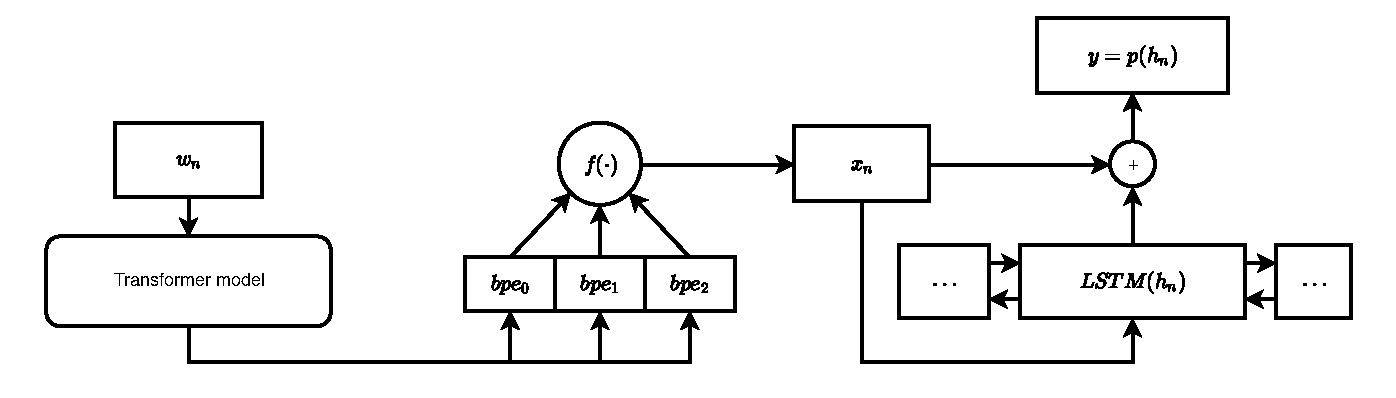
\includegraphics[scale=0.5]{single-step-final.pdf}
        \caption{\label{fig:model} Model outline for one input. A word
     $w_n$ is tokenized into $k$ BPE tokens by the transformer model,
     we then calculate a weighted sum over the layers for each feature
     embedding. The resulting embeddings are then passed to a BPE
     composition function $f$ that combines the $k$ different
     BPE embeddings into a word embedding. The word embedding is then
     passed to a LSTM followed by a dense prediction layer. }
	\end{figure}

	\subsubsection{Label smoothing}
    	Given that many of the languages have a large number of
     morphological tags, we want to prevent the model from growing
     overconfident for certain classes. To address this issue we
     introduce label smoothing \cite{szegedy2016rethinking}, that is,
     instead of the incorrect classes having $0\%$ probability and the
     correct class $100\%$ probability we let each of the incorrect
     classes have a small probability.

         Let $\alpha$ be our smoothing value, in our model we follow
     \citep{kondratyukstraka} and use $\alpha = 0.03$, and $C$ the
     number of classes, then given a one-hot encoded target vector $t$
     of size $C$, we calculate the smoothed probabilities as:
    \begin{equation}
        t_{smooth} = (1-\alpha)t + \frac{\alpha}{C}
    \end{equation}
    In words, we remove $\alpha$ from the correct class then
    distribute $\alpha$ uniformly among all classes.
     \subsection{Training}

     In our experiments we consider two possible training regimes. In
     the first regime we finetune the XLM-R models parameters, in the
     second regime we only extract weights for BPE tokens, that is, we
     use the model as a feature extractor. In all cases, we use
     end-to-end training.
     
                 When finetuning the model we freeze the XLM-R
     parameters for the first epoch, (effectively not finetuning at
     first).  When training the model we use a cosine annealing
     learning rate with restarts every epoch, that is, the learning
     rate starts high then incrementally decreases to
     $1\mathrm{e}{-12}$ over $N$ steps, where $N$ is the number of
     batches in an epoch.  We use the Adam optimizer, using standard
     parameters, with a learning rate of $0.001$ for layer importance
     parameter ($w$ in \cref{sec:bpe-features}),
    \begin{wraptable}{r}{4.8cm}
		\centering
		\begin{tabular}{lr} \\
			Parameter & Value \\
			\hline
			Epochs & 15 \\
			Batch size & 4 / 32 \\
			%Character representation size & 128 \\
            Word LSTM size & 768 \\
            Linear transform size & 1536 \\
			% optimizers
			Optimizer & Adam \\
			Learning rate & 0.001 \\
			Learning rate$_{xlmr}$ & 1e-06 \\
			% regularization
            Weight decay & 0.05 \\
			Label smoothing & 0.03 \\
            % described in text
            %Prediction dropout & 0.5 \\
			%Transformer dropout & 0.4 \\
            %Layer dropout & 0.1 \\
            %Input dropour & 0.2 \\
            %BPE dropout & 0.4 \\
            %Character dropout & 0.4 \\
		\end{tabular}
    		\caption{\label{tab:parameters} Hyperparameters used for
     training the model. Slashed indicate the value of a parameter
     when we finetune or extract features.}
	\end{wraptable}
        the parameters of the word LSTM, classification layer, and BPE
     combination module (when an RNN is used).  For the transformer
     parameters, we use a lower learning rate of $1\mathrm{e}{-6}$. We
     summarize the hyperparameters used in \cref{tab:parameters}.

            As an additional regularization in addition to weight
     decay and adaptive learning rate, we use dropout througout the
     model.  Generally, we apply dropoout before some feature is
     computed. We summarize the dropout as:

    \begin{enumerate}
        \item The first thing our model does is compute features
     for each BPE-token, we replac 20 percent of the BPE tokens with
     \texttt{<UNK>}.
        \item Then, we compute a weighted sum of the layer
     representations, to regularize this we we apply dropout on layers
     with a probability of $0.1$, that is we set all representations
     in the layer to $0$.
        \item We then combine the BPE-features into word-features
     and apply a dropout of $0.4\%$, and pass these into the
     Word-LSTM.
            \item Before the contextualized representation is passed
     to the classification layer, we apply a dropout of $0.4\%$.
    \end{enumerate}
    
    %We apply dropout on
    % the input to the transformer, replacing 20 percent of the BPE
    % tokens with \texttt{<UNK>}. After we have extracted layer
    % features from the transformer we apply a dropout of $0.4$, and
    % before computing the weighted sum of layers we apply dropout on
    % layers with a probability of $0.1$, that is we set all
    % representations in the layer to $0$.
    %After the word-LSTM has
    % processed the sequence, but before the final prediction, we apply
    % a dropout of $0.5$.

	
	\section{Results}
	\label{results}

             Even though our aim is to compare the relative
     performance of various BPE combination methods rather than to
     improve on the state of the art in absolute terms, we compare our
     results against the baseline reported by
     \citet{mccarthy2019sigmorphon}. This comparison serves the
     purpose of checking that our system is generally sound.  In
     particular, the actual state of the art, as reported by
     \citet{mccarthy2019sigmorphon,kondratyuk2019cross}, uses treebank
     concatenation or other methods to incorporate information from
     all treebanks available in a language, which means that results
     are not reported on a strict per-treebank basis and thus our
     numbers are not directly comparable.
    
     The accuracy of our system is computed by checking the prediction
        of morphological tags. We report in \cref{tab:results_tokens}
        the result for each of the four different methods, and the
        two training regimes.

    \begin{table}%[h]
	%\small
	\centering
	\begin{tabular}{l|c|cccc|cccc}
		& & \multicolumn{4}{c}{Finetuning} & \multicolumn{4}{c}{Feature extraction} \\
		Treebank & Baseline & Fst & Sum & Mean & RNN & Fst & Sum & Mean & RNN \\
		\hline
		Basque-BDT      & .676 & .857 & .884 & .877 & \textbf{.901} & .759 & .789 & .780 & \textbf{.834} \\
		Finnish-TDT     & .751 & .961 & .958 & .960 & \textbf{.965} & .853 & .856 & .847 & \textbf{.899} \\
		Turkish-IMST    & .620 & .848 & .859 & .855 & \textbf{.884} & .742 & .741 & .735 & \textbf{.775} \\
		Estonian-EDT    & .740 & .956 & .955 & .955 & \textbf{.961} & .855 & .856 & .853 & \textbf{.901} \\
		Spanish-AnCora  & .842 & .977 & .977 & .977 & \textbf{.979} & .951 & .954 & .952 & \textbf{.962} \\
		Arabic-PADT     & .770 & .946 & .946 & .947 & \textbf{.951} & .920 & .923 & .920 & \textbf{.936} \\
		Czech-CAC       & .771 & .968 & .968 & .968 & \textbf{.975} & .863 & .887 & .881 & \textbf{.924} \\
		Polish-LFG      & .657 & .956 & .953 & .953 & \textbf{.959} & .828 & .844 & .840 & \textbf{.878} \\
        \hline
        Average         & .728 & .933 & .937 & .936 & \textbf{.946} & .846 & .856 & .851 & \textbf{.888} \\
	\end{tabular}
    	\caption{\label{tab:results_tokens} Accuracy for morphological
          tagging. We show scores both for finetuning the XLM-R model and
          bare BPE embeddings extraction.}
    \end{table}


                Our system performs better than the baseline. As a
     general trend we see that the RNN method tends to perform better
     than all other tested methods. This trend is consistent across
     both languages families (agglutinative and fusional) and
     training regimes showing that, while the advantage of the RNN is
     small, it occurs consistenty.
        %
        In general we find that finetuning yields higher accuracy than
        plain feature extraction, on average the difference is about $5.8$
        percentage points.  This difference is to be expected when
        finetuning has 250M more parameters tuned to the task than the
        feature extraction. % less than expected...
    
                Focusing on the finetuning regime only, we see the
     largest benefits of the RNN method for Basque with an increased
     performance of $3.25$ points, and Turkish ($2.7$ points) over
     using mean or averaging. The Fst method for Basque and Turkish
     performs much worse with a decrease of $4.4$ percentage points
     for Basque and $3.6$ points for Turkish with respect to the RNN method.
    %\jp{In this paragraph we don't know the reference for ``increase'' or ``decrease''}
    %
        In the bare features extraction regime, we see a larger
     benefit for the RNN, of $3.7$ percentage points (Turkish) and
     $4.95$ points (Basque). Again, this is not unexpected: When
     finetuning the error rate is smaller, and therefore there is a
     smaller margin for a subsequent phase to yield and improvement.
    
  %  when
  %   fine-tuning the smaller error rate is overall smaller and
  %   therefore there is a smaller margin for a subsequent phase to
  %   yield an improvement.

    %We see again that the RNN performs
    %better than summation or averaging BPE embeddings.
    
	\begin{table}%[h]
	%\small
	\centering
	\begin{tabular}{l|cccc|cccc}
		 & \multicolumn{4}{c}{Finetuning} & \multicolumn{4}{c}{Feature extraction} \\
		Treebank & Fst & Sum & Mean & RNN & Fst & Sum & Mean & RNN  \\
		 \hline
		% agglutinative languages
        Basque-BDT      & .739 & .802 & .790 & \textbf{.835} & .657 & .715 & .703 & \textbf{.774} \\
		Finnish-TDT     & .940 & .946 & .946 & \textbf{.952} & .780 & .805 & .794 & \textbf{.861} \\ 
		Turkish-IMST    & .730 & .780 & .778 & \textbf{.818} & .653 & .683 & .664 & \textbf{.711} \\
		Estonian-EDT    & .938 & .939 & .939 & \textbf{.949} & .779 & .805 & .803 & \textbf{.868} \\
		% fusional languages
		Spanish-AnCora  & .956 & .961 & .959 & \textbf{.964} & .922 & .937 & .930 & \textbf{.947} \\
		Arabic-PADT     & .889 & .896 & .898 & \textbf{.907} & .902 & .909 & .906 & \textbf{.923}\\
		Czech-CAC       & .940 & .947 & .947 & \textbf{.959} & .786 & .849 & .840 & \textbf{.900} \\
		Polish-LFG      & .917 & .920 & .918 & \textbf{.927} & .696 & .761 & .752 & \textbf{.812} \\
        \hline
        Average         & .881 & .899 & .897 & \textbf{.913} & .772 & .808 & .799 & \textbf{.849} \\
	\end{tabular}
    \caption{\label{tab:results_large_tokens} Accuracy for
     morphological tagging on all tokens that are composed of 2 or
     more BPE tokens.}
\end{table}

        \Cref{tab:results_tokens} reports average accuracy for every word,
    thus also including those which are only composed of a single BPE
    token. To highlight the strengths and weaknesses of each
    composition method, we also compute the accuracy for longer words only 
    (composed of two BPE tokens or more). The results can be seen in
    \cref{tab:results_large_tokens}.
            We see the same trend for accuracy on tokens that are
     composed of two or more BPE tokens, as in the overall accuracy,
     where the RNN outperforms all other methods. We
     can also see that the average increase in accuracy when using an
     RNN is larger. This holds both when finetuning or extract bare features.
    %
        Given that the number of BPE tokens per word varies in the
     different languages, we also look at the accuracy of the
     different methods given the number of BPE tokens. We show
     per-language performance with the different methods in
     \cref{fig:bpe_lens}.
    
	\begin{figure}%[h!]
  	\centering
    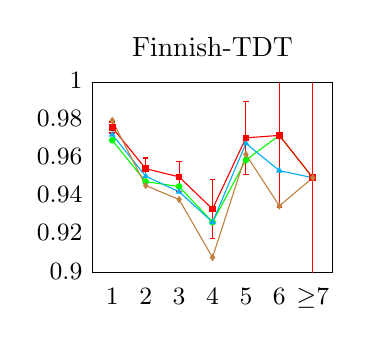
\begin{tikzpicture} 
	\begin{axis}[
	name=,
	title={Finnish-TDT},
    xtick style={draw=none},
    ytick style={draw=none},
    xtick={1,2,3,4,5,6,7},
    xticklabels={1,2,3,4,5,6,$\ge$7},
	typeset ticklabels with strut,
	legend pos=south west,
	ymajorgrids=false,
        ymax=1.0,
        ymin={0.9},
	grid style=dashed,
	height=4cm
	]
		\addplot[
		color=green,
		mark=*,
                mark size=1,
                error bars/.cd, y dir=both, y explicit,
		]
		coordinates {
			(1, 0.969671597)
			(2, 0.94797361)
			(3, 0.945349627)
			(4, 0.926686217)
			(5, 0.959302326)
			(6, 0.972222222)
			(7, 0.95)
};
		\addplot[
		color=cyan,
		mark=triangle*,
                mark size=1,
                error bars/.cd, y dir=both, y explicit,
		]
		coordinates {
			(1, 0.972648618)
			(2, 0.950801131)
			(3, 0.94263408)
			(4, 0.926686217)
			(5, 0.968023256)
			(6, 0.953703704)
			(7, 0.95)
};
		\addplot[
		color=red,
		mark=square*,
                mark size=1,
                error bars/.cd, y dir=both, y explicit,
		]
		coordinates {
			(1, 0.976369895)+=(0,0.00288107757099608)-=(0,0.00288107757099608)
			(2, 0.954759661)+=(0,0.005610028700870861)-=(0,0.005610028700870861)
			(3, 0.950441276)+=(0,0.007875906986290072)-=(0,0.007875906986290072)
			(4, 0.933528837)+=(0,0.01540785138661897)-=(0,0.01540785138661897)
			(5, 0.970930233)+=(0,0.019118549510097702)-=(0,0.019118549510097702)
			(6, 0.972222222)+=(0,0.03801018391614076)-=(0,0.03801018391614076)
			(7, 0.95)+=(0,0.08447212917485333)-=(0,0.08447212917485333)
};
		\addplot[
		color=brown,
		mark=diamond*,
                mark size=1,
                error bars/.cd, y dir=both, y explicit,
		]
		coordinates {
			(1, 0.980091171)
			(2, 0.945900094)
			(3, 0.93856076)
			(4, 0.908113392)
			(5, 0.962209302)
			(6, 0.935185185)
			(7, 0.95)
};

        \end{axis}
	\end{tikzpicture}
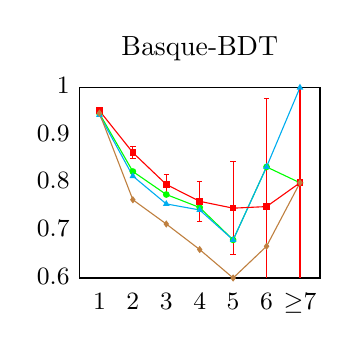
\begin{tikzpicture} 
	\begin{axis}[
	name=,
	title={Basque-BDT},
        xtick style={draw=none},
        ytick style={draw=none},
        xtick={1,2,3,4,5,6,7},
        xticklabels={1,2,3,4,5,6,$\ge$7},
	typeset ticklabels with strut,
	legend pos=south west,
	ymajorgrids=false,
        ymax=1.0,
        ymin={0.6},
	grid style=dashed,
	height=4cm
	]
		\addplot[
		color=green,
		mark=*,
                mark size=1,
                error bars/.cd, y dir=both, y explicit,
		]
		coordinates {
			(1, 0.945468053)
			(2, 0.823694905)
			(3, 0.775357386)
			(4, 0.748051948)
			(5, 0.68)
			(6, 0.833333333)
			(7, 0.8)
};
		\addplot[
		color=cyan,
		mark=triangle*,
                mark size=1,
                error bars/.cd, y dir=both, y explicit,
		]
		coordinates {
			(1, 0.942496285)
			(2, 0.814004376)
			(3, 0.755616065)
			(4, 0.742857143)
			(5, 0.68)
			(6, 0.833333333)
			(7, 1.0)
};
		\addplot[
		color=red,
		mark=square*,
                mark size=1,
                error bars/.cd, y dir=both, y explicit,
		]
		coordinates {
			(1, 0.95141159)+=(0,0.005148305118481129)-=(0,0.005148305118481129)
			(2, 0.863394811)+=(0,0.01190991764618752)-=(0,0.01190991764618752)
			(3, 0.796460177)+=(0,0.020591939005449287)-=(0,0.020591939005449287)
			(4, 0.761038961)+=(0,0.0425432420184802)-=(0,0.0425432420184802)
			(5, 0.746666667)+=(0,0.09746065981141003)-=(0,0.09746065981141003)
			(6, 0.75)+=(0,0.22787810036435233)-=(0,0.22787810036435233)
			(7, 0.8)+=(0,0.31002797388117415)-=(0,0.31002797388117415)
};
		\addplot[
		color=brown,
		mark=diamond*,
                mark size=1,
                error bars/.cd, y dir=both, y explicit,
		]
		coordinates {
			(1, 0.946210996)
			(2, 0.764301344)
			(3, 0.713410483)
			(4, 0.65974026)
			(5, 0.6)
			(6, 0.666666667)
			(7, 0.8)
};

        \end{axis}
	\end{tikzpicture}
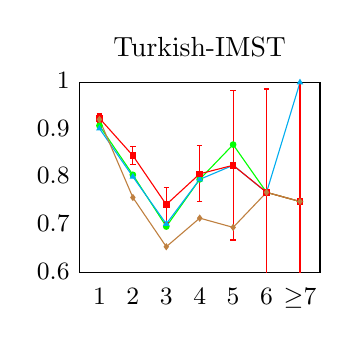
\begin{tikzpicture} 
	\begin{axis}[
	name=,
	title={Turkish-IMST},
        xtick style={draw=none},
        ytick style={draw=none},
        xtick={1,2,3,4,5,6,7},
        xticklabels={1,2,3,4,5,6,$\ge$7},
	typeset ticklabels with strut,
	legend pos=south west,
	ymajorgrids=false,
        ymax=1.0,
        ymin={0.6},
	grid style=dashed,
	height=4cm
	]
		\addplot[
		color=green,
		mark=*,
                mark size=1,
                error bars/.cd, y dir=both, y explicit,
		]
		coordinates {
			(1, 0.909405655)
			(2, 0.806088683)
			(3, 0.697416974)
			(4, 0.796511628)
			(5, 0.869565217)
			(6, 0.769230769)
			(7, 0.75)
};
		\addplot[
		color=cyan,
		mark=triangle*,
                mark size=1,
                error bars/.cd, y dir=both, y explicit,
		]
		coordinates {
			(1, 0.903346797)
			(2, 0.802117803)
			(3, 0.70295203)
			(4, 0.796511628)
			(5, 0.826086957)
			(6, 0.769230769)
			(7, 1.0)
};
		\addplot[
		color=red,
		mark=square*,
                mark size=1,
                error bars/.cd, y dir=both, y explicit,
		]
		coordinates {
			(1, 0.924985574)+=(0,0.008789990590271397)-=(0,0.008789990590271397)
			(2, 0.846459298)+=(0,0.018197041939921957)-=(0,0.018197041939921957)
			(3, 0.743542435)+=(0,0.03671374756645732)-=(0,0.03671374756645732)
			(4, 0.808139535)+=(0,0.058966217953330555)-=(0,0.058966217953330555)
			(5, 0.826086957)+=(0,0.15686382857803416)-=(0,0.15686382857803416)
			(6, 0.769230769)+=(0,0.21719589193854613)-=(0,0.21719589193854613)
			(7, 0.75)+=(0,0.3383902260894284)-=(0,0.3383902260894284)
};
		\addplot[
		color=brown,
		mark=diamond*,
                mark size=1,
                error bars/.cd, y dir=both, y explicit,
		]
		coordinates {
			(1, 0.922388921)
			(2, 0.75843812)
			(3, 0.65498155)
			(4, 0.715116279)
			(5, 0.695652174)
			(6, 0.769230769)
			(7, 0.75)
};

        \end{axis}
	\end{tikzpicture}
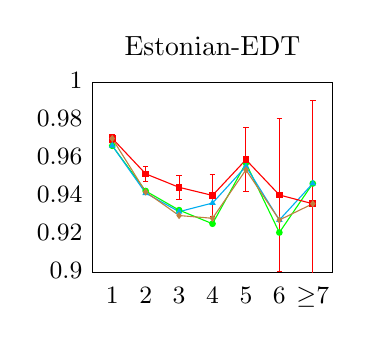
\begin{tikzpicture} 
	\begin{axis}[
	name=,
	title={Estonian-EDT},
        xtick style={draw=none},
        ytick style={draw=none},
        xtick={1,2,3,4,5,6,7},
        xticklabels={1,2,3,4,5,6,$\ge$7},
	typeset ticklabels with strut,
	legend pos=south west,
	ymajorgrids=false,
        ymax=1.0,
        ymin={0.9},
	grid style=dashed,
	height=4cm
	]
		\addplot[
		color=green,
		mark=*,
                mark size=1,
                error bars/.cd, y dir=both, y explicit,
		]
		coordinates {
			(1, 0.966596057)
			(2, 0.94286927)
			(3, 0.93281916)
			(4, 0.925671812)
			(5, 0.957522124)
			(6, 0.921052632)
			(7, 0.946808511)
};
		\addplot[
		color=cyan,
		mark=triangle*,
                mark size=1,
                error bars/.cd, y dir=both, y explicit,
		]
		coordinates {
			(1, 0.96667753)
			(2, 0.941765705)
			(3, 0.932007307)
			(4, 0.936535163)
			(5, 0.955752212)
			(6, 0.927631579)
			(7, 0.946808511)
};
		\addplot[
		color=red,
		mark=square*,
                mark size=1,
                error bars/.cd, y dir=both, y explicit,
		]
		coordinates {
			(1, 0.970506762)+=(0,0.002118846172644754)-=(0,0.002118846172644754)
			(2, 0.951867572)+=(0,0.0038703455288459482)-=(0,0.0038703455288459482)
			(3, 0.944793992)+=(0,0.006393466972485876)-=(0,0.006393466972485876)
			(4, 0.94053745)+=(0,0.011154986451904374)-=(0,0.011154986451904374)
			(5, 0.959292035)+=(0,0.01681968549237994)-=(0,0.01681968549237994)
			(6, 0.940789474)+=(0,0.04007961692831919)-=(0,0.04007961692831919)
			(7, 0.936170213)+=(0,0.05404871299247627)-=(0,0.05404871299247627)
};
		\addplot[
		color=brown,
		mark=diamond*,
                mark size=1,
                error bars/.cd, y dir=both, y explicit,
		]
		coordinates {
			(1, 0.970425289)
			(2, 0.942359932)
			(3, 0.929977674)
			(4, 0.928530589)
			(5, 0.953982301)
			(6, 0.927631579)
			(7, 0.936170213)
};

        \end{axis}
	\end{tikzpicture}
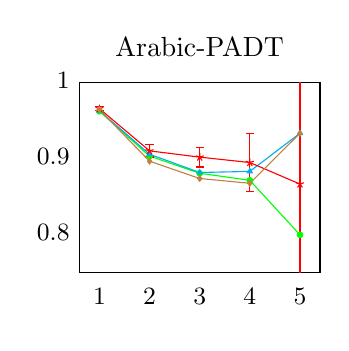
\begin{tikzpicture} 
	\begin{axis}[
	name=,
	title={Arabic-PADT},
        xtick style={draw=none},
        ytick style={draw=none},
        xtick={1,2,3,4,5,6,7},
        xticklabels={1,2,3,4,5,6,$\ge$7},
	typeset ticklabels with strut,
	legend pos=south west,
	ymajorgrids=false,
        ymax=1.0,
        ymin={0.75},
	grid style=dashed,
	height=4cm
	]
		\addplot[
		color=green,
		mark=*,
                mark size=1,
                error bars/.cd, y dir=both, y explicit,
		]
		coordinates {
			(1, 0.96220714)
			(2, 0.903356247)
			(3, 0.880846873)
			(4, 0.871595331)
			(5, 0.8)
};
		\addplot[
		color=cyan,
		mark=triangle*,
                mark size=1,
                error bars/.cd, y dir=both, y explicit,
		]
		coordinates {
			(1, 0.962904425)
			(2, 0.90578245)
			(3, 0.88183161)
			(4, 0.883268482)
			(5, 0.933333333)
};
		\addplot[
		color=red,
		mark=star,
                mark size=1.5,
                error bars/.cd, y dir=both, y explicit,
		]
		coordinates {
			(1, 0.965600595)+=(0,0.0024381283986652067)-=(0,0.0024381283986652067)
			(2, 0.910230489)+=(0,0.007976150815817857)-=(0,0.007976150815817857)
			(3, 0.90201871)+=(0,0.012961727810939487)-=(0,0.012961727810939487)
			(4, 0.894941634)+=(0,0.03810358069342934)-=(0,0.03810358069342934)
			(5, 0.866666667)+=(0,0.18330014190315588)-=(0,0.18330014190315588)
};
		\addplot[
		color=brown,
		mark=diamond*,
                mark size=1,
                error bars/.cd, y dir=both, y explicit,
		]
		coordinates {
			(1, 0.964298996)
			(2, 0.896684189)
			(3, 0.873953717)
			(4, 0.86770428)
			(5, 0.933333333)
};

        \end{axis}
	\end{tikzpicture}
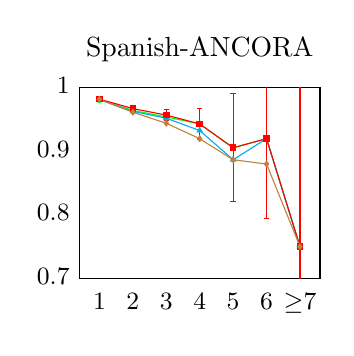
\begin{tikzpicture} 
	\begin{axis}[
	name=,
	title={Spanish-ANCORA},
        xtick style={draw=none},
        ytick style={draw=none},
        xtick={1,2,3,4,5,6,7},
        xticklabels={1,2,3,4,5,6,$\ge$7},
	typeset ticklabels with strut,
	legend pos=south west,
	ymajorgrids=false,
        ymax=1.0,
        ymin={0.7},
	grid style=dashed,
	height=4cm
	]
		\addplot[
		color=green,
		mark=*,
                mark size=1,
                error bars/.cd, y dir=both, y explicit,
		]
		coordinates {
			(1, 0.981325799)
			(2, 0.96449483)
			(3, 0.954242928)
			(4, 0.943152455)
			(5, 0.905660377)
			(6, 0.92)
			(7, 0.75)
};
		\addplot[
		color=cyan,
		mark=triangle*,
                mark size=1,
                error bars/.cd, y dir=both, y explicit,
		]
		coordinates {
			(1, 0.981233921)
			(2, 0.962999875)
			(3, 0.952163062)
			(4, 0.932816537)
			(5, 0.886792453)
			(6, 0.92)
			(7, 0.75)
};
		\addplot[
		color=red,
		mark=square*,
                mark size=1,
                error bars/.cd, y dir=both, y explicit,
		]
		coordinates {
			(1, 0.982267549)+=(0,0.0012411463013903851)-=(0,0.0012411463013903851)
			(2, 0.967360159)+=(0,0.0038992019513958173)-=(0,0.0038992019513958173)
			(3, 0.957154742)+=(0,0.008154258951432975)-=(0,0.008154258951432975)
			(4, 0.943152455)+=(0,0.023764512705614565)-=(0,0.023764512705614565)
			(5, 0.905660377)+=(0,0.08501108280383891)-=(0,0.08501108280383891)
			(6, 0.92)+=(0,0.1250821627692161)-=(0,0.1250821627692161)
			(7, 0.75)+=(0,0.3383902260894284)-=(0,0.3383902260894284)
};
		\addplot[
		color=brown,
		mark=diamond*,
                mark size=1,
                error bars/.cd, y dir=both, y explicit,
		]
		coordinates {
			(1, 0.981991915)
			(2, 0.9616295)
			(3, 0.944259567)
			(4, 0.919896641)
			(5, 0.886792453)
			(6, 0.88)
			(7, 0.75)
};

        \end{axis}
	\end{tikzpicture}
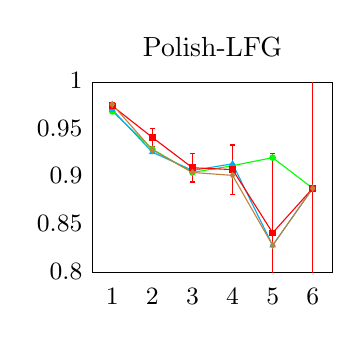
\begin{tikzpicture} 
	\begin{axis}[
	name=,
	title={Polish-LFG},
        xtick style={draw=none},
        ytick style={draw=none},
        xtick={1,2,3,4,5,6,7},
        xticklabels={1,2,3,4,5,6,$\ge$7},
	typeset ticklabels with strut,
	legend pos=south west,
	ymajorgrids=false,
        ymax=1.0,
        ymin={0.8},
	grid style=dashed,
	height=4cm
	]
		\addplot[
		color=green,
		mark=*,
                mark size=1,
                error bars/.cd, y dir=both, y explicit,
		]
		coordinates {
			(1, 0.969714687)
			(2, 0.930019881)
			(3, 0.905500705)
			(4, 0.912601626)
			(5, 0.921052632)
			(6, 0.888888889)
};
		\addplot[
		color=cyan,
		mark=triangle*,
                mark size=1,
                error bars/.cd, y dir=both, y explicit,
		]
		coordinates {
			(1, 0.971468662)
			(2, 0.926838966)
			(3, 0.907616361)
			(4, 0.914634146)
			(5, 0.828947368)
			(6, 0.888888889)
};
		\addplot[
		color=red,
		mark=square*,
                mark size=1,
                error bars/.cd, y dir=both, y explicit,
		]
		coordinates {
			(1, 0.975444341)+=(0,0.0032933193579321087)-=(0,0.0032933193579321087)
			(2, 0.942345924)+=(0,0.009152642925086161)-=(0,0.009152642925086161)
			(3, 0.910437236)+=(0,0.014925424898063413)-=(0,0.014925424898063413)
			(4, 0.908536585)+=(0,0.025763757285900076)-=(0,0.025763757285900076)
			(5, 0.842105263)+=(0,0.08322533572401784)-=(0,0.08322533572401784)
			(6, 0.888888889)+=(0,0.22927231782530055)-=(0,0.22927231782530055)
};
		\addplot[
		color=brown,
		mark=diamond*,
                mark size=1,
                error bars/.cd, y dir=both, y explicit,
		]
		coordinates {
			(1, 0.977081384)
			(2, 0.929224652)
			(3, 0.905500705)
			(4, 0.902439024)
			(5, 0.828947368)
			(6, 0.888888889)
};

        \end{axis}
	\end{tikzpicture}
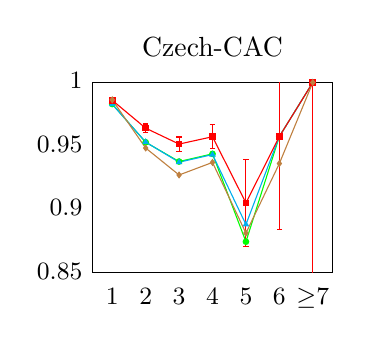
\begin{tikzpicture} 
	\begin{axis}[
	name=,
	title={Czech-CAC},
        xtick style={draw=none},
        ytick style={draw=none},
        xtick={1,2,3,4,5,6,7},
        xticklabels={1,2,3,4,5,6,$\ge$7},
	typeset ticklabels with strut,
	legend pos=south west,
	ymajorgrids=false,
        ymax=1.0,
        ymin={0.85},
	grid style=dashed,
	height=4cm
	]
		\addplot[
		color=green,
		mark=*,
                mark size=1,
                error bars/.cd, y dir=both, y explicit,
		]
		coordinates {
			(1, 0.983029434)
			(2, 0.952917936)
			(3, 0.937731522)
			(4, 0.943788645)
			(5, 0.874576271)
			(6, 0.957446809)
			(7, 1.0)
};
		\addplot[
		color=cyan,
		mark=triangle*,
                mark size=1,
                error bars/.cd, y dir=both, y explicit,
		]
		coordinates {
			(1, 0.982858704)
			(2, 0.953082558)
			(3, 0.937202328)
			(4, 0.943226532)
			(5, 0.888135593)
			(6, 0.957446809)
			(7, 1.0)
};
		\addplot[
		color=red,
		mark=square*,
                mark size=1,
                error bars/.cd, y dir=both, y explicit,
		]
		coordinates {
			(1, 0.986000137)+=(0,0.00134856026285523)-=(0,0.00134856026285523)
			(2, 0.964029961)+=(0,0.003317290752570475)-=(0,0.003317290752570475)
			(3, 0.951490563)+=(0,0.005607453201193778)-=(0,0.005607453201193778)
			(4, 0.95727937)+=(0,0.009489989645509947)-=(0,0.009489989645509947)
			(5, 0.905084746)+=(0,0.03403245585016136)-=(0,0.03403245585016136)
			(6, 0.957446809)+=(0,0.07333263763454309)-=(0,0.07333263763454309)
			(7, 1.0)+=(0,0.3367274202349047)-=(0,0.3367274202349047)
};
		\addplot[
		color=brown,
		mark=diamond*,
                mark size=1,
                error bars/.cd, y dir=both, y explicit,
		]
		coordinates {
			(1, 0.986341597)
			(2, 0.948390814)
			(3, 0.927147645)
			(4, 0.937043283)
			(5, 0.881355932)
			(6, 0.936170213)
			(7, 1.0)
};

        \end{axis}
	\end{tikzpicture}

         \caption{\label{fig:bpe_lens} Per-language accuracy on tokens
     with different numbers of BPE components, for the finetuning
     training regime. The last data point on the $x$-axis refers to
     all tokens composed of seven or more BPE tokens.  We indicate the
     method by encoding {\color{brown} Fst as brown}, {\color{green} summation as green}, {\color{blue} averaging as
     blue} and {\color{red} RNN as red}. The accuracy is given on the $y$-axis. We
     show the the Agresti-Coull approximation of a 95\%-confidence
     interval for the RNN method \citep{agresti1998approximate}.  We
     do not show the intervals for other methods to avoid excessive
     clutter.}
	\end{figure}

	
	
	\section{Discussion}

%    \subsection{BPE composition methods}
    % For our experiments
    % We see that
        For morphological feature prediction, the RNN method is more
     effective than the other proposed methods (summing, averaging or
     taking the first BPE token). This holds regardless of training
     regime (finetuning versus feature extraction) and across
     languages with different BPE per word ratios.
    
                 As we see it, the advantage of the RNN over
     commutative methods (Sum, Mean) and taking the first BPE token is
     that it can take the order of elements into account. In broad
     terms, information about the order of elements in morphology
     allows a system to determine what is a stem, prefix, or suffix.
      Thus allowing a model to collect more predictive information
     from sub-word embeddings.

             We can suspect that the average BPE per word ratio in a
     language affects the performance of the composition method
     used. To further control this variable, in \cref{fig:scatter_len}
     we plot the average number of BPE tokens per word, and compare
     this average against the gain in accuracy yielded by using the
     RNN method over summation.  For finetuning we see that in
     general the average number of BPE tokens do not matter that
     much. The two cases where it does matter is for Turkish and
     Basque, where we see a substantial improvement of about $3$
     percentage points. We note however that these are also the
     languages with the lowest amount of training data.
    %
        For the other languages the improvements lie in the range $.6$
     to $1.2$ percentage points. This indicates that when finetuning,
     the model can provide information that allows commutative methods
     to properly compose BPE tokens. However, looking at bare feature
     extraction we see that there is a larger gap between the low
     BPE-ratio and the high BPE-ratio languages.
    %\adam{This indicates that while the
    % pretrained BPE weights contain predictive information, there is
    % still more to be extracted from them.}

        Our sample of languages contain both fusional and
     agglutinative languages, and the typology does not appear to have
     an effect in our experiments. We see about the same trends for
     the fusional languages with a high BPE-to-token ratio as the
     agglutinative languages.

    %%%%%%%%
    %     We suspect this might be influenced by how the task was
    % setup, with using composite tags rather than multi-class
    % prediction.
    %   With only one prediction layer, the layer have to extract information for all classes 
    %If we were to use one prediction layer per
    % grammatical class, each layer would act independently of the
    % other layers, thus allowing for an explicit mapping of BPE tokens
    % to grammatical classes.
    
    %\adam{Effect of training data?}
    %\adam{This may be influenced by our choice of creating composite tags instead of predicting each feature individually.}

    \subsection{Fst method}

            The idea behind the Fst method is that the transformer is
     sufficiently powerful to pool the relevant information into the
     first BPE token.
    %
                            However, our experiments reveal that it is
     less efficient than any other method we tested for morphological
     sequence classification across languages. We see in
     \cref{tab:results_tokens} that the method is, on average, $.4$
     and $1$ percentage points lower than the next lowest scoring
     method for finetuning and feature extraction respectively.
     % We see that
             This effect is further enhanced when we consider the
     accuracy of words composed of more than two BPE token in
     \cref{tab:results_large_tokens}, where the difference is $1.6$
     and $2.7$ points, compared against the next lowest scoring
     method, for finetuning and feature extraction repescively. When
     we compare the performance against the RNN this difference only
     increases, showing a gain of $3.2$ percentage points and $7.7$
     points for finetuning and feature extraction respectively.

                         While the Fst method may be effective,
     primarily because of the expressivity of the transformer
     architecture, the method forces the model to push the predictive
     information of several BPE tokens into the first one. This adds
     an implicit objective to the model which is not strictly
     necessary, since we can pool this information, and appear to
     degrade the performance.
     %
    % This present 

    \subsection{Sum and Mean}
                When we consider the commutative methods of combining
     BPE embeddings, summation or averaging, we see no clear advantage
     for either of them over the other one, when doing
     finetuning. However, when extracting features only we see hints
     that summation is more effective than averaging. For feature
     extraction, summation is $.5$ percentage points better than
     averaging, and words composed of two or more BPE tokens exhibit
     an advantage of $.9$ point for summation.
    
                This discrepancy suggests that by averaging, we are
     removing some predictive information from the pretrained BPE
     tokens, that is, by reducing the values in the BPE embeddings
     uniformly across a sequence of BPE embeddings we lose useful
     information.
        We believe that some BPE embeddings contain more predictive
     information than others, and by summing them we retain all the
     information.
      %
                     But when we finetune, the differense between
     summing and averaging almost disapear, the model appears to learn
     how to distribute the information uniformly across the BPE tokens
     that compose a word, and is thus able to retain the information
     better. Interestingly, the model learns distribute the
     information across multiple BPE tokens more efficiently than
     pushing the information into the first token. This is shown by
     the large difference in accuracy between finetuning and feature extraction
     for the Fst and averaging method.
   
\begin{figure}%{r}{8cm}
    \centering  
        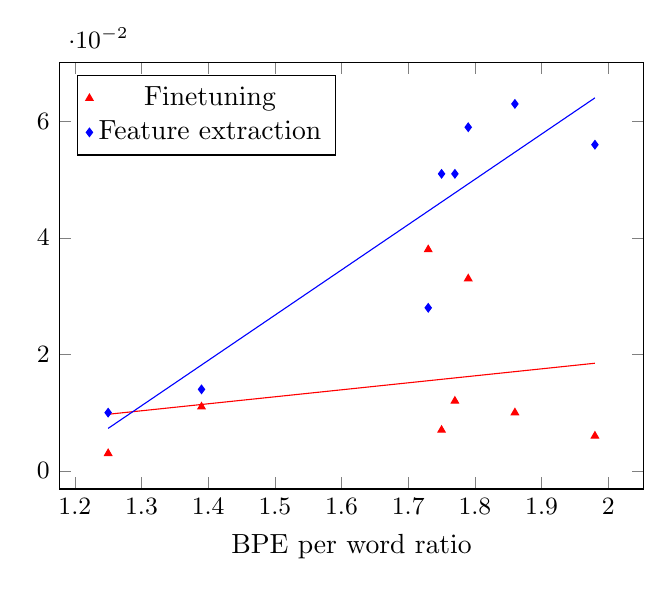
\begin{tikzpicture}
    	\begin{axis}[
		name=,
		title={},
		height=7cm,
        width=9cm,
        legend pos=north west,
        xlabel={BPE per word ratio},
		]
            \addplot[
             color=red,
    	     mark=triangle*,
    	     only marks,
              mark size=1.5
    	     ]
        	 coordinates {
            (1.98,0.006000000000000005)
            (1.79,0.03299999999999992)
            (1.73,0.03799999999999992)
            (1.86,0.010000000000000009)
            (1.39,0.01100000000000001)
            (1.25,0.0030000000000000027)
            (1.75,0.007000000000000006)
            (1.77,0.01200000000000001)
            };
            \addlegendentry{Finetuning}
    
            \addplot[no marks, color=red] table [row sep=\\,y={create col/linear regression={y=Y}},forget plot] {
            X Y \\
            1.98 0.006000000000000005 \\
            1.79 0.03299999999999992 \\
            1.73 0.03799999999999992 \\
            1.86 0.010000000000000009 \\
            1.39 0.01100000000000001 \\
            1.25 0.0030000000000000027 \\
            1.75 0.007000000000000006 \\
            1.77 0.01200000000000001 \\
            };
    
            \addplot[
             color=blue,
    	     mark=diamond*,
    	     only marks,
              mark size=1.5
    	     ]
            coordinates {
            (1.98,0.05599999999999994)
            (1.79,0.05900000000000005)
            (1.73,0.027999999999999914)
            (1.86,0.06299999999999994)
            (1.39,0.014000000000000012)
            (1.25,0.009999999999999898)
            (1.75,0.051000000000000045)
            (1.77,0.051000000000000045)
            };
            \addlegendentry{Feature extraction}
    
            \addplot[no marks, color=blue] table [row sep=\\,y={create col/linear regression={y=Y}},forget plot] {
            X Y \\
            1.98 0.05599999999999994 \\
            1.79 0.05900000000000005 \\
            1.73 0.027999999999999914 \\
            1.86 0.06299999999999994 \\
            1.39 0.014000000000000012 \\
            1.25 0.009999999999999898 \\
            1.75 0.051000000000000045 \\
            1.77 0.051000000000000045 \\
            };
    %\legend{Finetuning, Feature extraction}
        	\end{axis}
        \end{tikzpicture}
        \caption{The difference in accuracy between summation and RNN plotted against average number of BPE
     tokens per word in all languages, with a linear regression line.}
    \label{fig:scatter_len}
    \end{figure}

    \section{Parameterization of Fst, Sum and Mean}

        One question that arises when we look at
     \cref{fig:bpe_lens}, specifically considering the performance on
     tokens composed of only one BPE token, is whether this is due to
     the additional parameters in the RNN model, or the added
     contextual information of the words. We would expect that for the
     words with only one BPE token, the performance of the model would
     be the same for all methods. But for practical reasons we push
     all tokens through an RNN, effectively doing a non-linear
     transformation with $\mathsf{tanh}$ activations on the tokens
     composed of only one BPE token.
    %
                Typically, the difference in accuracy between various
     method for length one token words is small (barely visible in
     \cref{fig:bpe_lens}). But for example in Finnish we see a larger
     difference. Although, in general if we perform better on longer
     tokens consisting of BPE tokens that also appear as words in the
     data, we could also expect the performance to be better for
     tokens of BPE length one, because we will have more accurarate
     representations of the contextual words.

            We test this by parameterizing the Fst, Sum, and Mean
     method. This is sone by adding a non-linear transformation with
     $\mathsf{ReLU}$ activation before we compute the Sum, Mean, or
     select the first BPE-token.


        \begin{table}%[h]
	%\small
	\centering
	\begin{tabular}{l|c|cccc|cccc}
		& & \multicolumn{4}{c}{Finetuning} & \multicolumn{4}{c}{Feature extraction} \\
		Treebank & Baseline & Fst & Sum & Mean & RNN & Fst & Sum & Mean & RNN \\
		\hline
		Basque-BDT      & .676 & .857 & .884 & .877 & \textbf{.901} & .759 & .793 & .794 & \textbf{.834} \\
		Finnish-TDT     & .751 & .961 & .958 & .960 & \textbf{.965} & .853 & .856 & .855 & \textbf{.899} \\
		Turkish-IMST    & .620 & .848 & .859 & .855 & \textbf{.884} & .742 & .722 & .729 & \textbf{.775} \\
		Estonian-EDT    & .740 & .956 & .955 & .955 & \textbf{.961} & .855 & .856 & .853 & \textbf{.901} \\
		Spanish-AnCora  & .842 & .977 & .977 & .977 & \textbf{.979} & .951 & .954 & .952 & \textbf{.962} \\
		Arabic-PADT     & .770 & .946 & .946 & .947 & \textbf{.951} & .920 & .923 & .920 & \textbf{.936} \\
		Czech-CAC       & .771 & .968 & .968 & .968 & \textbf{.975} & .863 & .887 & .881 & \textbf{.924} \\
		Polish-LFG      & .657 & .956 & .953 & .953 & \textbf{.959} & .828 & .844 & .840 & \textbf{.878} \\
        \hline
        Average         & .728 & .933 & .937 & .936 & \textbf{.946} & .846 & .856 & .851 & \textbf{.888} \\
	\end{tabular}
    	\caption{\label{tab:parameters} The accuracy of morphological tagging when we let the fst, sum and mean method use a linear transformation layer.}
    
    \end{table}

    \section{Conclusions and Future Work}


    %    In colcusion, our results show that composing word
    % representations using an RNN from BPE tokens is more effective
    % than summation, averaging or taking the first BPE token.  This
    % have implications for systems that use pretrained models with BPE
    % tokenization that perform some type of word classification. 
    
                In conclusion, our results indicate that using an RNN
     to compose word representations from BPE tokens is more efficient
     than two commutative methods, summing and averaging, and also
     more effective than letting a transformer model automatically pool the
     predictive word-level information into a single BPE token.
    %
    We show this for the task of morphological sequence classification in 
     eight different languages with varying morphology and BPE
     lengths, aswell as for two training regimes, finetuning and
     feature extraction.

    % consequences for probing?
    % Lexical probes om pretrained word-embeddings using the Fst model will be bad.
    
     
    In future work we want to continue experimenting with the different
    BPE composition methods, specifically looking at more complex
    syntactic and semantic tasks, such as dependency and/or
    constituency parsing, semantic role labeling and named entity recognition. 
    %
        We also wish to run our experiments on the hundreds
     of available UD treebanks to improve the robustness of our
     results.  
    
%	\section*{Acknowledgments}

	% include your own bib file like this:
	\bibliographystyle{coling}
	\bibliography{coling2020}
	
\end{document}
